\documentclass[12pt]{article}
\usepackage{cite}
\usepackage{color}
\usepackage{graphicx}
\usepackage{caption}
\usepackage{subcaption}

\title{LCMS Chromatogram Smoothing With Generative Adversarial Networks}

\author{Gabriel Ferns(CS Senior) , Max Horowitz-Gelb(CS Senior)}

\begin{document}

\maketitle

\abstract{
Liquid Chromatography Mass Spectrometry is a powerful tool for identifying and quantifying proteins in a complex sample. High throughput methods of LCMS such as DIA\cite{DIA} allow for analysis of samples with thousands of proteins. But this increase in throughput comes at the cost of a decrease in signal quality. This gives incentive for post extraction methods to clean and smooth chromatogram signal data. Here , using a new and powerful deep learning framework known as GANs \cite{GAN}, we attempt to smooth chromatograms, without distortion of the true underlying quantifiable data. 
\color{red}
Highlight results here
\color{black}
}

\section{Introduction}
DIA \cite{DIA} is a method of LCMS for quanitifying thousands of proteins. In order to to do analyze thousands of proteins at the same time, DIA methods have one cycling through thousands of different m/z windows, where each window is used to quantify a single peptide. Because we are analyzing so many windows at each time, the dwell time, or time in which signal is extracted, must be very short. Because of this, the quality of the data extracted can be quite poor. An alternative to DIA is SRM, or Selected Reaction Monitoring,\cite{SRM}. SRM is not good for quantifying more than a handful of peptides at a time, but the data generated is of far superior quality to DIA.

\begin{figure}
\centering
\begin{subfigure}{.5\textwidth}
  \centering
  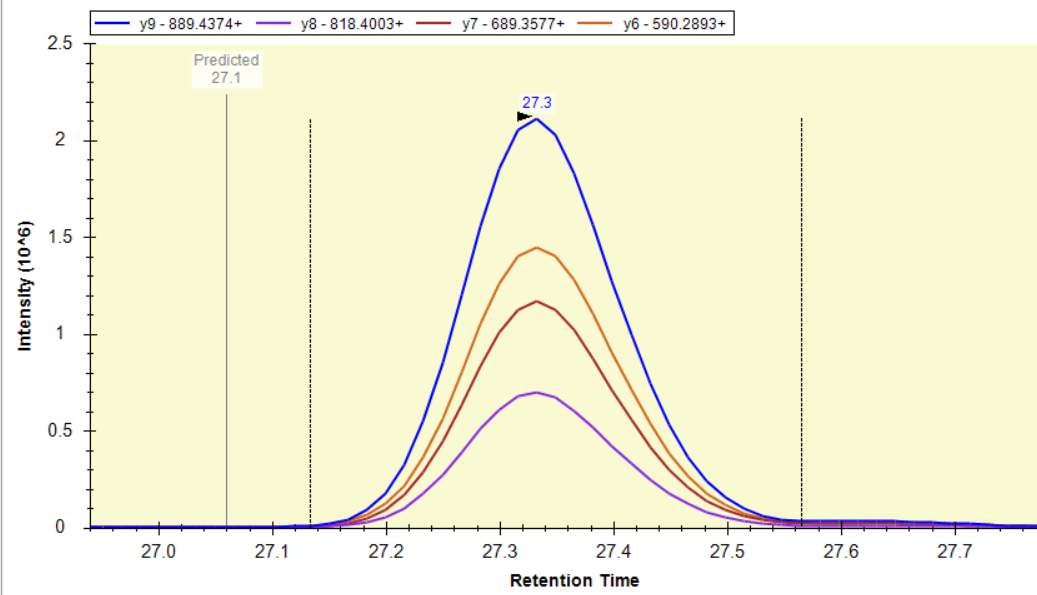
\includegraphics[width=1\linewidth]{SRM_example}
  \caption{SRM Chromatogram}
  \label{fig:sub1}
\end{subfigure}%
\begin{subfigure}{.5\textwidth}
  \centering
  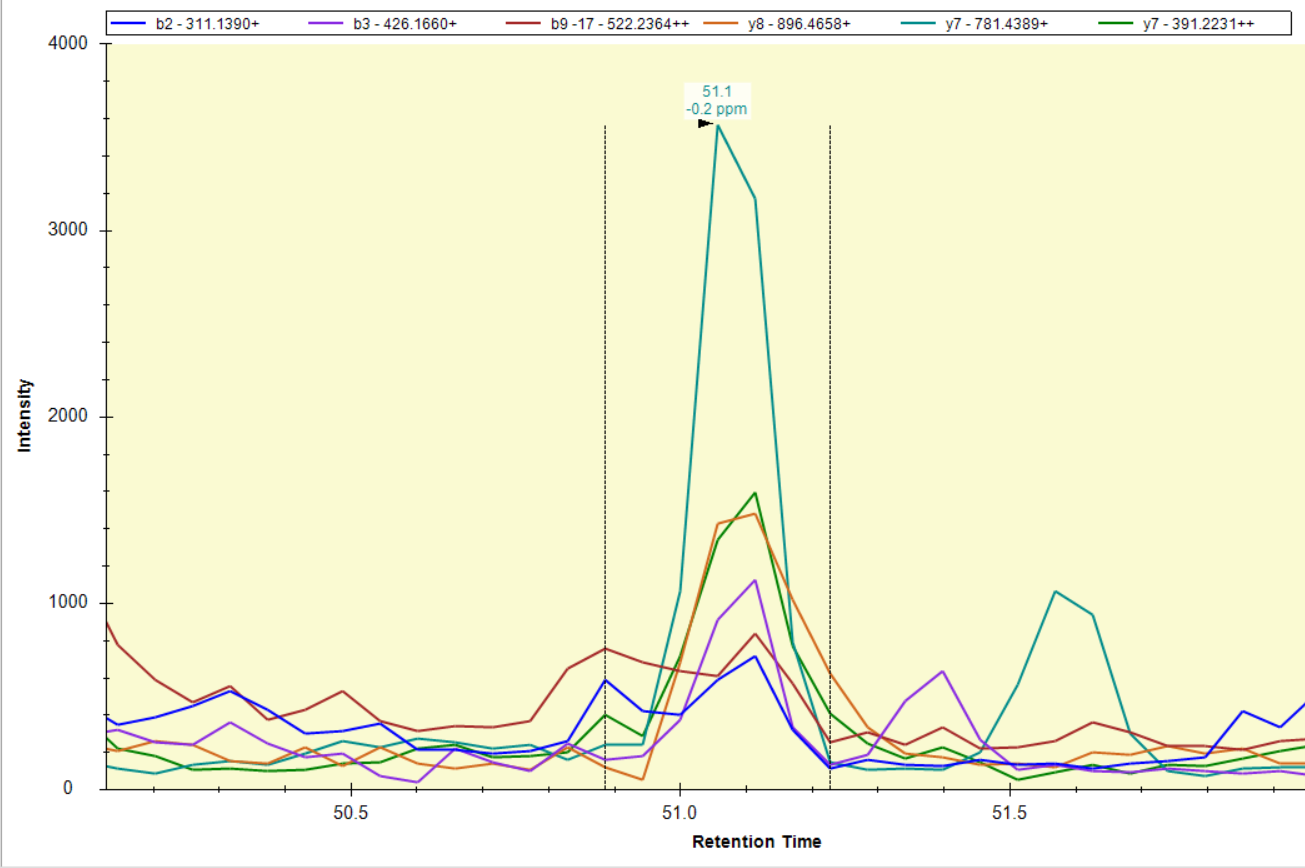
\includegraphics[width=1\linewidth]{DIA_example}
  \caption{DIA Chromatogram}
  \label{fig:sub2}
\end{subfigure}
\caption{Here we show two chromatograms. As one can see the noise and the smoothness is much better in the chromatogram coming from an SRM dataset.}
\label{fig:test}
\end{figure}

\section{Task Definition}
\section{Algorithm Definition}
\section{Methodology}
\section{Results}
\section{Discussion}
\section{Related Work}
\section{Future Work}
\section{Conclusion}

\bibliography{writeup}{}
\bibliographystyle{plain}

\end{document}